\documentclass[12pt]{article}
\input{Assignment-1-Data-Structures.tex}
\usepackage[utf8]{inputenc}
\usepackage[T1]{fontenc}
\usepackage[a4paper, left=2.4cm, right=2.4cm, top=2cm, bottom=2cm, nomarginpar]{geometry}
\usepackage{amsmath, algorithm, pgfplots, pgf, pdfpages, amsfonts, amssymb, stmaryrd, enumitem,graphicx, algpseudocode, setspace, listings, courier, color, caption, centernot, hyperref, lstautogobble, zi4, mathtools, lmodern, colortbl, array, multicol, fancyhdr, lastpage, svg}
\usepackage{booktabs}
\hypersetup{
    pdftitle={CE204_FP1_G6},
    pdftoolbar=true,        % show Acrobat’s toolbar?
    pdfmenubar=true,        % show Acrobat’s menu?
    pdfauthor={Muhammet Yağcıoğlu},
    pdfsubject={CE204_FP_RPs},
    pdfcreator={Muhammet Yağcıoğlu},   % creator of the document
    pdfproducer={Muhammet Yağcıoğlu}, % producer of the document
    colorlinks,
    linkcolor={black},
    citecolor={black},
    urlcolor={blue!80!black}
}
\usepackage[noblocks]{authblk}
\usepackage[version=4]{mhchem}
\usepackage[export]{adjustbox}
\usepackage{eso-pic} % Required for absolute positioning
\graphicspath{ {./images/} }
\usetikzlibrary{patterns}
\usepackage{tikz-3dplot}
\usepackage[version=4]{mhchem}
\usepackage[export]{adjustbox}
\usepgfplotslibrary{groupplots}
\usepackage{xcolor}
\usepackage[absolute,overlay]{textpos}
\usepackage{ragged2e}
\usepackage{xcolor}
\usepackage{amsthm}
\usepackage{tikz}




%----------compiler settings---------
\setlength{\parindent}{0pt}
\everymath{\displaystyle}
\onehalfspacing

%-----------colors----------
\pgfplotsset{compat=1.18}
\definecolor{bluekeywords}{rgb}{0.13, 0.13, 1}
\definecolor{greencomments}{rgb}{0, 0.5, 0}
\definecolor{redstrings}{rgb}{0.9, 0, 0}
\definecolor{graynumbers}{rgb}{0.5, 0.5, 0.5}
\definecolor{bronze}{rgb}{0.82, 0.41, 0.12}
\definecolor{crimson}{rgb}{0.86, 0.08, 0.24}
\definecolor{brown(web)}{rgb}{0.65, 0.16, 0.16}
\definecolor{darkspringgreen}{rgb}{0.16, 0.32, 0.75}
\definecolor{blue(ncs)}{rgb}{0.0, 0.53, 0.74}
\definecolor{amber}{rgb}{1.0, 0.49, 0.0}
\definecolor{cadmiumgreen}{rgb}{0.0, 0.42, 0.24}




%-------code frame-----------
\lstset{
    autogobble,
    columns=fullflexible,
    showspaces=false,
    showtabs=false,
    breaklines=true,
    showstringspaces=false,
    breakatwhitespace=true,
    escapeinside={(*@}{@*)},
    commentstyle=\color{greencomments},
    keywordstyle=\color{bluekeywords},
    stringstyle=\color{redstrings},
    numberstyle=\color{graynumbers},
    basicstyle=\ttfamily\footnotesize,
    frame=l,
    framesep=12pt,
    xleftmargin=12pt,
    tabsize=4,
    captionpos=b
}



\lstdefinelanguage{myMMA}{
keywords={SetDirectory, NotebookDirectory, Exp, IdentityMatrix, Eigenvalues, 
ListPlot, PlotRange, PlotStyle, Directive, PointSize, AspectRatio, Blue, Graphics, Line, 
Manipulate, Show, Sqrt, UniformDistribution, GammaDistribution, BetaDistribution, 
Nintegrate, For, DataRange, AxesLabel, PlotLabel, Transpose, Export, Plot, Append, Infinity},
keywordstyle=\color{black},
commentstyle=\color{gray}, 
identifierstyle=\color{blue},
sensitive=false,
comment=[l]{(*},
morecomment=[s]{/*}{*/},
morestring=[b]',
morestring=[b]"
}






%-----gauss declare---------
\pgfmathdeclarefunction{gauss}{2}{%
  \pgfmathparse{1/(#2*sqrt(2*pi)) * exp(-((x-#1)^2)/(2*#2^2))}%
}
\usetikzlibrary{arrows.meta, decorations.markings}
\pgfplotsset{compat=1.17}







%--------------page numbering------------
\fancyfoot[R]{page \thepage\ of \textcolor{bronze}{\pageref{LastPage}}}
\fancyhead[R]{Group 6}



%-------------qframe settings---------------

\usepackage[framemethod=TikZ]{mdframed}
\newmdenv[%
    skipabove=1em, % space above the frame
    skipbelow=1em, % space below the frame
    linewidth=1pt, % width of the frame lines
    linecolor=gray!80, % color of the frame lines
    backgroundcolor=gray!9, % background color inside the frame
    roundcorner=5pt, % radius of the rounded corners
    innerleftmargin=1em, % margin within the frame at the left
    innerrightmargin=1em, % margin within the frame at the right
    innertopmargin=0.5em, % margin within the frame at the top
    innerbottommargin=0.5em % margin within the frame at the bottom
]{qframe}

\newenvironment{q}
{
    \begin{qframe}
    \noindent\textit{\textbf{Problem Statement:}}
    \par\smallskip
}
{
    \end{qframe}
}





%-------------ANSWER TAG---------------
\newcommand{\AnswerTag}{\hfill 
\begin{tikzpicture} \fill[black] (0.35cm,0) -- (0,0.175cm) -- (0.35cm,0.35cm) -- cycle;\end{tikzpicture}}



%-------Theorem and another question frames----------
\newenvironment{theorem}{\begin{mdframed}\textbf{Theorem.}}{\end{mdframed}}

%usage: \begin{theorem}

\newenvironment{question}{\begin{mdframed}\textbf{Question.}}{\end{mdframed}}

%usage: %usage: \begin{question}
\fancyhead[L]{Assignment 2 - Discrete Random Variables}
\author{adzetto}
\everymath{\displaystyle}
\usepackage{hyperref} 

\begin{document}
\maketitle\thispagestyle{fancy}

\pagestyle{fancy}
\tableofcontents
\newpage
\section*{Problem 1. Coin Spins (\#Probability)}
\addcontentsline{toc}{section}{Problem 1}

One day you overhear how two fellow students discuss a show in which a performer spins a coin many mes, resulting in Tails 30 mes in a row. You hear them discussing:

\textbf{Yueh Han}: "That outcome would be extremely unlikely with fair coins. They must be using trick coins (maybe double-tailed coins), or the experiment must have been rigged somehow (maybe with magnets)."

\textbf{Akma}: "It's true that the string TT . . T of length 30 is very unlikely; the chance is $(1 / 2)^{30} \approx$ $9 \times 10^{-10}$ with fair coins. But any other specific string of $H$ and $T$ with length 30 has exactly the same probability! The reason the outcome seems extremely unlikely is that the number of possible outcomes grows exponen ally as the number of spins grows, so any outcome would seem extremely unlikely. You could just as well have made the same argument even without looking at the results of their experiment, which means you really don't have evidence against the coins being fair."

Help Yueh Han and Akma resolve their debate.

\begin{q}
1. Discuss the conversation of Yueh Han and Akma. With whom do you agree and why?
\end{q}


\textit{Answer.}

\textbf{Statistical Inference and Probability Analysis}

Consider a random variable \( X \) representing the outcome of a coin toss, where \( X = 1 \) denotes tails and \( X = 0 \) denotes heads. The probability space is defined as \( \Omega = \{0, 1\} \) with a probability measure \( P \) such that \( P(X=1) = p \) and \( P(X=0) = 1-p \). In the context of fair coins, \( p = \frac{1}{2} \).

Yueh Han posits that the occurrence of 30 consecutive tails (denoted as \( T^{30} \)) suggests a non-random process, implicating the coin might not be fair. This hypothesis considers the cumulative probability of the event \( T^{30} \) under the assumption of a fair coin, which is computed as \( P(T^{30}| \text{Fair}) = \left(\frac{1}{2}\right)^{30} \).

Akma, however, argues from a standpoint of equiprobability of all sequences of length 30 in the sample space \( \Omega^{30} \). For any sequence \( s \in \Omega^{30} \), \( P(s) = \left(\frac{1}{2}\right)^{30} \). Thus, the specific sequence \( T^{30} \) is not statistically significant from this perspective.

\newpage
\textbf{Resolution of the Debate.}

I agree with Yueh Han.

Yueh Han's argument is based on the intuitive improbability of seeing an exceptionally uncommon occurrence while assuming a fair coin, which is a valid issue in actual settings. However, Akma's logic is consistent with basic probabilistic concepts, emphasising the equal probability of all particular sequences of the same length. The essence of the problem is how these probabilities are interpreted and contextualised.

In conclusion, Yueh Han's argument has value in a practical, statistical inference environment, where seeing an exceptionally unusual occurrence may rise to questions about the underlying assumptions (such as coin fairness). While Akma's reasoning is theoretically correct, it may ignore practical aspects of statistical analysis.


\begin{q}
2. Suppose there are only two models: either the coins are all fair (and spun fairly), or double-tailed coins are being used in which case the probability of Tails is 1 . Let \(p\) be the prior probability that the coins are fair. Find the posterior probability that the coins are fair, given that they landed Tails in 30 out of 30 trials.
\end{q}

\textit{Answer.}

Let \( p \) represent the prior probability that the coin is fair. The hypothesis \( H_0 \) states that the coin is fair, implying \( P(T | H_0) = \left(\frac{1}{2}\right)^{30} \), where \( T \) denotes the event of observing 30 tails in 30 flips. The alternative hypothesis \( H_1 \) posits the coin is double-tailed, yielding \( P(T | H_1) = 1 \). The total probability of observing \( T \), denoted \( P(T) \), is the sum of probabilities under both hypotheses, weighted by their respective prior probabilities. Thus, \( P(T) = p \cdot P(T | H_0) + (1 - p) \cdot P(T | H_1) \).

Bayes' Theorem stipulates:

\[
P(H_0 | T) = \frac{P(T | H_0) \cdot P(H_0)}{P(T)},
\]

Substituting the known values, we obtain:

\[
P(H_0 | T) = \frac{\left(\frac{1}{2}\right)^{30} \cdot p}{p \cdot \left(\frac{1}{2}\right)^{30} + (1 - p) \cdot 1},
\]

This fraction simplifies to:

\[
P(H_0 | T) = \frac{p \cdot \left(\frac{1}{2}\right)^{30}}{p \cdot \left(\frac{1}{2}\right)^{30} + 1 - p}.
\]

The posterior probability \( P(H_0 | T) \) represents our updated belief in the fairness of the coin after observing the data \( T \). This probability is contingent on the prior \( p \), reflecting the influence of initial beliefs in Bayesian inference.

\begin{q}
3. For which values of the prior, \(p\), is the posterior probability that the coins are fair greater than 0.5 ? (What does the prior need to be to make the fair-coin model more probable according to the posterior?)
\end{q}

\textit{Answer.}

Focusing on the inequality:

\[
P(H_0 | T) > 0.5,
\]

From the previous calculation, we recall that:

\[
P(H_0 | T) = \frac{p \cdot \left(\frac{1}{2}\right)^{30}}{p \cdot \left(\frac{1}{2}\right)^{30} + 1 - p},
\]

\[
\frac{p \cdot \left(\frac{1}{2}\right)^{30}}{p \cdot \left(\frac{1}{2}\right)^{30} + 1 - p} > 0.5.
\]

Solving this inequality will provide the range of \( p \) values for which the fair-coin model is more probable than not, given the observed data. The inequality can be transformed as follows:

\[
2 \cdot p \cdot \left(\frac{1}{2}\right)^{30} > p \cdot \left(\frac{1}{2}\right)^{30} + 1 - p,
\]

\[
p \cdot \left(\frac{1}{2}\right)^{30} > 1 - p,
\]
\[
p \cdot \left(\frac{1}{2}\right)^{30} + p > 1,
\]

\[
p \left(\left(\frac{1}{2}\right)^{30} + 1\right) > 1.
\]

Thus, solving for \( p \) gives:

\[
p > \frac{1}{\left(\frac{1}{2}\right)^{30} + 1} = \frac{1073741824}{1073741825} \approx 0.9999999990687 \cong 1. 
\]




\textbf{Interpretation of the Result.}

The outcome highlights how the prior probability significantly impacts the posterior probability, especially with extreme or unlikely data. In this scenario, observing 30 tails in a row is such a rare event under the assumption of a fair coin (probability \( \left(\frac{1}{2}\right)^{30} \)) that to still believe the coin is fair, one must have an almost absolute prior conviction in its fairness.


\newpage
\section*{Problem 2. Medical test (\#Probability)}
\addcontentsline{toc}{section}{Problem 2}
Omer wants to be really certain about a diagnosis so he takes a series of \(n\) identical medical tests. He hopes multiple tests will reduce his uncertainty.

Events:
\begin{itemize}
    \item[-] \(D\) : Omer has the disease being tested for.
    \item[-]  \(T_j\) : Omer tests positive on the \(j^{\text {th }}\) test for \(j=1,2, \ldots, n\).
\end{itemize}

Let \(p=P(D)\) be the prior probability that he has the disease.

\begin{q}
1. Assume for this part the test results are conditionally independent given Omer's disease status. Let \(a_0=P\left(T_j \mid D\right)\) and \(b_0=P\left(T_j \mid D^c\right)\), where \(a_0\) and \(b_0\) don't depend on \(j\). Find the posterior probability that Omer has the disease, given that he tests positive on all \(n\) of the \(n\) tests. (Hint: Since \(a_0\) does not depend on \(j\) (the index of a test result), the algebra simplifies a lot since \(P\left(T_i \mid D\right) P\left(T_j \mid D\right)=a_0^2\) for any test indices \(i\) and \(j\). The same holds for \(b_0\).)
\end{q}
\textit{Answer.}

Let \( \Omega \) be the sample space for Omer's health condition and test results. Define \( D \in \Omega \) as the event that Omer has the disease and \( D^c \) as its complement. Further, let \( T_j \in \Omega \) for \( j = 1, 2, \ldots, n \) represent the event of a positive result in the \( j^\text{th} \) test. The problem posits a prior probability \( P(D) = p \), and it is given that \( P(T_j \mid D) = a_0 \) and \( P(T_j \mid D^c) = b_0 \) for all \( j \), with \( a_0 \) and \( b_0 \) independent of \( j \). 

The task is to determine the posterior probability \( P(D \mid \bigcap_{j=1}^n T_j) \). By Bayes' theorem, this is expressed as:

\[ P(D \mid \bigcap_{j=1}^n T_j) = \frac{P(\bigcap_{j=1}^n T_j \mid D) P(D)}{P(\bigcap_{j=1}^n T_j)} \]

Under the assumption of conditional independence given \( D \) or \( D^c \), one has 

\[ P(\bigcap_{j=1}^n T_j \mid D) = \prod_{j=1}^n P(T_j \mid D) = a_0^n \]
\[ P(\bigcap_{j=1}^n T_j \mid D^c) = \prod_{j=1}^n P(T_j \mid D^c) = b_0^n \]

The denominator, \( P(\bigcap_{j=1}^n T_j) \), is evaluated using the law of total probability:

\[ P(\bigcap_{j=1}^n T_j) = P(D)P(\bigcap_{j=1}^n T_j \mid D) + P(D^c)P(\bigcap_{j=1}^n T_j \mid D^c) \]
\[ = pa_0^n + (1-p)b_0^n \]

Substituting these into Bayes' theorem gives:

\[ P(D \mid \bigcap_{j=1}^n T_j) = \frac{a_0^n p}{pa_0^n + (1-p)b_0^n}. \]

\begin{q}
2. Suppose some people have a gene that makes them always test positive on this type of medical test. Let \(G\) be the event that Omer has the gene. Assume that \(P(G)=1 / 2\) and that \(D\) and \(G\) are independent - that is, the gene does not make you more or less susceptible to the disease. If Omer has the gene, he'll test positive on all \(n\) tests. If Omer does not have the gene, then the test results are conditionally independent given his disease status. Let \(a_1=P\left(T_j \mid D, G^c\right)\) and \(b_1=P\left(T_j \mid D^c, G^c\right)\), where \(a_1\) and \(b_1\) don't depend on \(j\). Now, suppose that Omer tests positive on all \(n\) tests and find the posterior probability that Omer has the disease.
\end{q}
\textit{Answer.}

We are tasked with computing \(P(D \mid \bigcap_{j=1}^n T_j)\). To achieve this, we first express \(P(\bigcap_{j=1}^n T_j)\) via the law of total probability, conditioning on \(G\) and \(G^c\):

\[ P(\bigcap_{j=1}^n T_j) = P(G)P(\bigcap_{j=1}^n T_j \mid G) + P(G^c)P(\bigcap_{j=1}^n T_j \mid G^c). \]

Given \(P(G) = \frac{1}{2}\) and \(P(\bigcap_{j=1}^n T_j \mid G) = 1\) (since possessing \(G\) guarantees positive test results), we have:

\[ P(\bigcap_{j=1}^n T_j) = \frac{1}{2} + \frac{1}{2}P(\bigcap_{j=1}^n T_j \mid G^c). \]

Under the condition \(G^c\), the tests are conditionally independent with respect to \(D\) and \(D^c\), yielding:

\[ P(\bigcap_{j=1}^n T_j \mid G^c) = P(D)P(\bigcap_{j=1}^n T_j \mid D, G^c) + P(D^c)P(\bigcap_{j=1}^n T_j \mid D^c, G^c). \]

Given \(a_1 = P(T_j \mid D, G^c)\) and \(b_1 = P(T_j \mid D^c, G^c)\), and exploiting the conditional independence, we deduce:

\[ P(\bigcap_{j=1}^n T_j \mid G^c) = pa_1^n + (1-p)b_1^n. \]

Substituting this into our expression for \(P(\bigcap_{j=1}^n T_j)\), we obtain:

\[ P(\bigcap_{j=1}^n T_j) = \frac{1}{2} + \frac{1}{2}(pa_1^n + (1-p)b_1^n). \]

By Bayes' theorem, the posterior probability \(P(D \mid \bigcap_{j=1}^n T_j)\) is:

\[ P(D \mid \bigcap_{j=1}^n T_j) = \frac{P(\bigcap_{j=1}^n T_j \mid D)P(D)}{P(\bigcap_{j=1}^n T_j)}. \]

As \(P(\bigcap_{j=1}^n T_j \mid D)\) involves both cases where \(G\) is present and absent, we have:

\[ P(\bigcap_{j=1}^n T_j \mid D) = P(G)P(\bigcap_{j=1}^n T_j \mid D, G) + P(G^c)P(\bigcap_{j=1}^n T_j \mid D, G^c) = \frac{1}{2} + \frac{1}{2}a_1^n. \]

Finally,

\[ P(D \mid \bigcap_{j=1}^n T_j) = \frac{(\frac{1}{2} + \frac{1}{2}a_1^n)p}{\frac{1}{2} + \frac{1}{2}(pa_1^n + (1-p)b_1^n)}. \]
\newpage
\begin{q}
3. Using the same setup as in part (2.), find the posterior probability that Omer has the gene given that he tests positive on all \(n\) of the tests.
\end{q}
\textit{Answer.}

\[ P(G \mid \bigcap_{j=1}^n T_j) = \frac{P(\bigcap_{j=1}^n T_j \mid G)P(G)}{P(\bigcap_{j=1}^n T_j)}. \]

We already know from the setup that \( P(G) = \frac{1}{2} \) and \( P(\bigcap_{j=1}^n T_j \mid G) = 1 \) because the presence of the gene guarantees positive results in all tests. The denominator \( P(\bigcap_{j=1}^n T_j) \) was calculated in part (2) as:

\[ P(\bigcap_{j=1}^n T_j) = \frac{1}{2} + \frac{1}{2}(pa_1^n + (1-p)b_1^n). \]

So,

\[ P(G \mid \bigcap_{j=1}^n T_j) = \frac{1 \times \frac{1}{2}}{\frac{1}{2} + \frac{1}{2}(pa_1^n + (1-p)b_1^n)} \]
\[ = \frac{\frac{1}{2}}{\frac{1}{2} + \frac{1}{2}(pa_1^n + (1-p)b_1^n)}. \]
\[ P(G \mid \bigcap_{j=1}^n T_j) = \frac{1}{1 + pa_1^n + (1-p)b_1^n}. \]


\newpage
\section*{Problem 3. Proofreading (\#Distributions, \#ModelSelection)}
\addcontentsline{toc}{section}{Problem 3}

Problem 3. Proofreading (\#Distributions, \#ModelSelection)

A book has \(n\) typos. Two proofreaders, Sho and Haruna, independently read the book. Sho finds each typo independently with probability \(p_1\), and Haruna with probability \(p_2\). Let \(X_1\) be the number of typos caught by Sho, \(X_2\) be the number caught by Harua, and \(X\) be the number caught by at least one of the two proofreaders.

\begin{q}
1. Find the distribution of \(X\). Motivate your answer.
\end{q}
\textit{Answer.}

Let \( X \) be defined as the number of typos caught by at least one of the two proofreaders, Sho and Haruna. We consider a single typo within the book. The event that Sho finds this typo has probability \( p_1 \), and the event that Haruna finds it has probability \( p_2 \). The events are independent, hence the probability that neither Sho nor Haruna finds the typo is \( (1 - p_1)(1 - p_2) \). Therefore, the probability that at least one of them finds the typo is \( 1 - (1 - p_1)(1 - p_2) \), which simplifies to \( p_1 + p_2 - p_1p_2 \). Denote this probability as \( q \), so \( q = p_1 + p_2 - p_1p_2 \).

We now consider the collection of all \( n \) typos in the book. The probability that a specific set of \( k \) typos is found by at least one proofreader, while the remaining \( n - k \) typos are not found by either, is given by \( q^k(1 - q)^{n-k} \). Since there are \( \binom{n}{k} \) distinct ways to choose \( k \) typos from \( n \), the probability of exactly \( k \) typos being found by at least one proofreader is \( \binom{n}{k} q^k (1 - q)^{n-k} \). Thus, \( X \) follows a binomial distribution with parameters \( n \) and \( q \), denoted by \( X \sim \text{Binomial}(n, q) \).


\begin{q}
2. Assuming \(p_1=p_2\), find the conditional distribution of \(X_1\) given that \(X_1+X_2=t\). That is, if we know \(t\) typos were found, how many were found by the first proofreader? (Hint: \(X_1+X_2 \neq X\). Note that we are conditioning on the number of typos found by Sho plus the number found by Haruna. This is not the same as the number of typos found by at least one of the two proofreaders - we are double-counting the typos found by both of them.)
\end{q}
\textit{Answer.}

Firstly, the probability that Sho finds exactly \(k\) typos and Haruna finds \(t-k\) typos can be computed under the binomial distribution framework. Since \(X_1\) and \(X_2\) are independent and identically distributed, we have \(X_1 \sim \text{Binomial}(n, p)\) and \(X_2 \sim \text{Binomial}(n, p)\). The probability of Sho finding exactly \(k\) typos is given by the binomial formula as \(P(X_1=k) = \binom{n}{k} p^k (1-p)^{n-k}\), and similarly for Haruna, \(P(X_2=t-k) = \binom{n}{t-k} p^{t-k} (1-p)^{n-(t-k)}\).

The probability of the combined event \(X_1=k\) and \(X_1+X_2=t\) is the product of these probabilities due to their independence, which yields:
\[
P(X_1=k, X_1+X_2=t) = \binom{n}{k} p^k (1-p)^{n-k} \cdot \binom{n}{t-k} p^{t-k} (1-p)^{n-(t-k)}.
\]

Next, we consider the probability \(P(X_1+X_2=t)\). This is the probability that a total of \(t\) typos are found by both proofreaders combined. Since the proofreaders are independent and identically distributed, the total number of typos found follows a binomial distribution with parameters \(2n\) and \(p\), giving us \(P(X_1+X_2=t) = \binom{2n}{t} p^t (1-p)^{2n-t}\).

Therefore, the conditional probability \(P(X_1=k \mid X_1+X_2=t)\) is obtained by dividing the joint probability by the marginal probability:
\[
P(X_1=k \mid X_1+X_2=t) = \frac{\binom{n}{k} p^k (1-p)^{n-k} \cdot \binom{n}{t-k} p^{t-k} (1-p)^{n-(t-k)}}{\binom{2n}{t} p^t (1-p)^{2n-t}}.
\]

Upon simplification, where terms involving \(p\) and \(1-p\) cancel out, we arrive at:
\[
P(X_1=k \mid X_1+X_2=t) = \frac{\binom{n}{k} \binom{n}{t-k}}{\binom{2n}{t}}.
\]
\newpage
\begin{q}
3. You write a book with 100,000 words. On average, you make a typo once every 300 words. Sho and Haruna proofread your book. Sho finds 299 typos while Haruna finds 314 typos. Use model selection to decide whether Haruna is better than Sho at finding typos or whether it is just a coincidence that she found more than Sho this time.
Hints:
\begin{itemize}
\item[-] Follow the frequentist model selection recipe from the Session 12 Study Guide.
\item[-] For the null model, think carefully about which distribution to use for the number of typos that exist in the book.
\item[-] You'll need your answer to part (2.) above.
\item[-] You will need to implement a simulation for this problem. Don't rely on looking up a known distribution of the test statistic.
\end{itemize}
\end{q}
\textit{Answer.}

Let \(\Omega\) denote the sample space representing all possible outcomes of the typo detection process. For each typo in the manuscript, a proofreader either identifies it (success) or overlooks it (failure). Given \(n = 333\) (the estimated number of typos in the manuscript), the sample space \(\Omega\) is structured as the Cartesian product of individual typo detection events, i.e., \(\Omega = \{0,1\}^n\). We define two random variables \(X_1, X_2 : \Omega \rightarrow \mathbb{Z}^+\), where \(X_1(\omega)\) and \(X_2(\omega)\) represent the number of typos identified by Sho and Haruna, respectively, for an outcome \(\omega \in \Omega\). Under the null hypothesis \(H_0\), these random variables are identically distributed according to a binomial distribution, \(X_i \sim \text{Bin}(n, p)\), where \(p\) is the common probability of detecting a typo, estimated as \(\frac{299 + 314}{2 \times 333} \approx 0.9204\). To simulate this stochastic process, we employ Monte Carlo methods, generating a large number \(N\) of random samples \(\{\omega_1, \omega_2, \ldots, \omega_N\}\) from \(\Omega\). For each \(\omega_i\), we compute \(X_1(\omega_i)\) and \(X_2(\omega_i)\), and subsequently their sum \(S_i = X_1(\omega_i) + X_2(\omega_i)\). Our focal interest lies in the conditional distribution of \(X_1\) given \(S = 613\), derived in the previous question:

\[ P(X_1 = k \mid S = 613) = \frac{\binom{n}{k} \binom{n}{613 - k}}{\binom{2n}{613}}. \]

Given this conditional probability, the simulation iterates over a range of values \(k \in \{0, 1, \ldots, n\}\), calculating \(P(X_1 = k \mid S = 613)\) at each step. The p-value is then computed as:

\[ \text{p-value} = \sum_{k=0}^{299} P(X_1 = k \mid S = 613). \]

This p-value represents the probability, under \(H_0\), of Sho detecting an equal or lesser number of typos than the observed 299.



\begin{figure}[ht!]
    \centering
    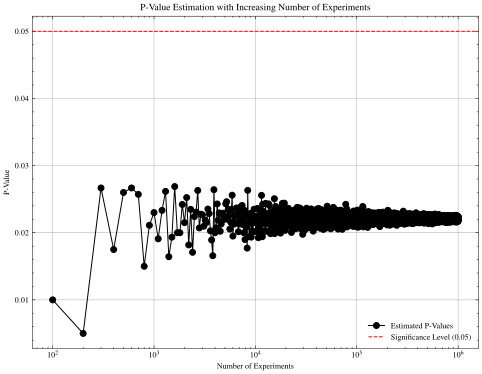
\includegraphics{myimage.eps}
    \caption{}
    \label{fig:enter-label}
\end{figure}


The Monte Carlo simulation yielded p-values of 0.0217 for 10,000 trials and 0.02146 for 100,000 trials, indicating a tendency to reject the null hypothesis \(H_0\). The null hypothesis in this instance is that Sho and Haruna have identical typo detection skills. The p-values are smaller than the standard significance threshold of 0.05, indicating that the observed difference in the number of typos discovered by Sho and Haruna is statistically significant. This suggests that Haruna's greater detection rate of typos than Sho's is unlikely to be due to random fluctuation or chance.


\newpage

\subsection*{Algorithm and Code}

\begin{algorithm}
\caption{P-Value Estimation with Increasing Number of Experiments}
\begin{algorithmic}[1]

\State \textbf{Define:} 
\State \indent $\Omega \gets \text{Sample space of a Bernoulli trial}$
\State \indent $\mathcal{F} \gets \sigma\text{-algebra of events}$
\State \indent $\mathbb{P} \gets \text{Probability measure}$
\State \indent $X: \Omega \to \{0, 1, \dots, n\} \gets \text{Random variable for Bernoulli trial}$
\State \indent $p \in [0,1] \gets \text{Success probability}$
\State \indent $t \in \{0, 1, \dots, 2n\} \gets \text{Observed number of successes in } 2n \text{ trials}$
\State \indent $\mathcal{N} \gets \{100, 101, \dots, 999999\} \gets \text{Manifold of experiment counts}$

\State \textbf{Compute conditional probability $p_k$:}
\State \indent $p_k = \binom{n}{k} p^k (1-p)^{n-k} \frac{\binom{n}{t-k} p^{t-k} (1-p)^{n-(t-k)}}{\binom{2n}{t} p^t (1-p)^{2n-t}}$

\State \textbf{Calculate p-value:}
\State \indent $p_{\text{value}} = \sum_{k=0}^{299} p_k$

\State \textbf{For each} $n \in \mathcal{N}$:
\State \indent \textbf{Sample} $X_1, X_2, \dots, X_n \sim \sum_{k=0}^n p_k \delta_k$
\State \indent $\hat{p}_{\text{value}}(n) \gets \frac{1}{n} \sum_{i=1}^n \mathbb{I}[X_i \leq 299]$

\State \textbf{Plotting:}
\State \indent Plot $(n, \hat{p}_{\text{value}}(n))$ with logarithmic scale on x-axis
\State \indent Add horizontal line at $y = 0.05$ for significance level
\State \indent Label axes and add title
\State \indent Display plot

\end{algorithmic}
\end{algorithm}
\begin{lstlisting}[language=Python]
import numpy as np
import matplotlib.pyplot as plt
from scipy.stats import binom
import scienceplots
plt.style.use(['science', 'ieee'])

# Constants
n = 333
t = 613
p = (299 + 314) / (2 * n)

# Calculate conditional probabilities
prob_k = [binom.pmf(k, n, p) * binom.pmf(t - k, n, p) / binom.pmf(t, 2 * n, p) for k in range(n + 1)]

# Calculate p-value
p_value = sum(prob_k[:300])

# Simulation for different numbers of experiments
experiment_counts = [i for i in range(100, 1000001, 100)]
p_values = []

for exp_count in experiment_counts:
    counts = np.random.choice(np.arange(n + 1), size=exp_count, p=prob_k)
    p_values.append(np.mean(counts <= 299))

# Plotting
plt.figure(figsize=(8, 6))
plt.plot(experiment_counts, p_values, marker='o')
plt.axhline(y=0.05, color='r', linestyle='--', label='Significance Level (0.05)')
plt.xlabel('Number of Experiments')
plt.ylabel('P-Value')
plt.title('P-Value Estimation with Increasing Number of Experiments')
plt.xscale('log')
plt.legend()
plt.grid(True)
plt.show()
\end{lstlisting}

\begin{q}
4. Stretch goal. This part is entirely optional - there is no penalty for not attempting it and there is no penalty for getting it wrong if you choose to try it. If you provide a great, well-written solution to this problem, you will get an extra score of (5) on \#ParameterEstimation. If you fall short of a (5), you can still earn a (4) for a slightly flawed solution but the errors have to be minimal. You cannot score less than (4) on this problem - instead you will get no extra grade if the attempt is insufficient. This is a hard problem and it is possible that nobody will get it right.
Problem: Use the same setup as in part (3.) above but with the following additional information: of the 299 typos Sho found and the 314 Haruna found, 285 were found by both of them. This means Sho found \((299-285)=14\) typos that Haruna did not find and Haruna found \((314-285)=29\) typos that Sho did not find.
Question: How many typos are left in the book, found by neither Sho nor Haruna?
Task: Address this question by estimating all of the following unknown variables using Bayesian parameter estimation \(-p_1\) (the probability that Sho finds a typo), \(p_2\) (the probability that Haruna finds a typo), and \(t\) (the total number of typos in the book). You can then answer how many of the \(t\) typos were not found by either proofreader.
Why is this hard? We don't know for certain how many typos there are in the book! We only know how many were found by Sho or Haruna (or both) but not how many typos were not found by them. However, with everything we covered in class till now, you have enough tools to estimate the probabilities that the proofreaders find typos and therefore how many of the overall typos they found. Good luck!
\end{q}
\textit{Answer.}

Let \( t \) denote the total number of typos in the book. The observable variables are the number of typos found by Sho, \( t_{\text{Sho}} = 299 \), and by Haruna, \( t_{\text{Haruna}} = 314 \), with an overlap of \( t_{\text{both}} = 285 \) typos found by both. The challenge lies in estimating the latent variables \( p_1 \), \( p_2 \), and \( t \). We posit a Bayesian model where \( p_1 \), \( p_2 \), and \( t \) are treated as random variables with prior distributions reflecting our initial uncertainty about their values. Given the observed data \( D = \{ t_{\text{Sho}}, t_{\text{Haruna}}, t_{\text{both}} \} \), we seek the posterior distributions \( P(p_1 | D) \), \( P(p_2 | D) \), and \( P(t | D) \).

So, consider the parameter space \(\Theta \subseteq \mathbb{R}^3\), defined such that each element \(\theta = (p_1, p_2, t) \in \Theta\) represents the probabilities \(p_1, p_2 \in [0, 1]\) and the total number of typos \(t \in \mathbb{Z}^+\). The uniform distributions \(P(p_1)\) and \(P(p_2)\) over [0, 1] reflect absence of initial bias. The parameter \(t\) follows a Poisson distribution with a rate parameter \(\lambda\), estimated from the average frequency of typos, yielding \(P(t) = \text{Poisson}(\lambda)\).

Define the likelihood function \( \mathcal{L}(D | p_1, p_2, t) \), which quantifies the probability of observing the data \( D \) given specific values of \( p_1 \), \( p_2 \), and \( t \). This likelihood is a complex function owing to the dependencies between the variables and the nature of the overlapping detections by Sho and Haruna.

The posterior distribution \(P(\Theta | \text{data})\) is proportional to the product of the likelihood and the prior distributions, incorporating the observed data. Utilizing an affine invariant ensemble-based MCMC method, we define an ensemble of walkers \(\vec{X} = (X_1, \ldots, X_L)\) in \(\mathbb{R}^{3L}\). Each walker follows a transition kernel \(\mu(d\tilde{x}_k, x_k | \vec{x}_{[k]})\) preserving the target distribution under affine transformations. The stretch move \(X_k(t) \rightarrow Y = X_j + Z(X_k(t) - X_j)\) is implemented, where \(Z\) is a scaling variable ensuring symmetric proposals and detailed balance.

Statistical tests are used to check if the MCMC chain is convergent and to make sure that the samples are a good representation of the posterior distribution. From these examples, we can guess what the posterior distributions of \(p_1\), \(p_2\), and \(t\) are. To get an idea of how many typos are still missing, we can use the formula \(Y = t \times (1 - p_1) \times (1 - p_2)\), which gives us an expected number of typos.

\newpage
\begin{lstlisting}[language=Python]
import emcee
import numpy as np
from scipy.stats import binom, poisson

# Observed data
n_Sho = 14
n_Haruna = 29
n_Both = 285

# Likelihood function
def likelihood(theta, n_Sho, n_Haruna, n_Both):
    p1, p2, t = theta
    # Probability of different outcomes
    prob_Sho = p1 * (1 - p2)
    prob_Haruna = p2 * (1 - p1)
    prob_Both = p1 * p2

    # Likelihood based on Binomial distribution
    likelihood = binom.pmf(n_Sho, t, prob_Sho) * binom.pmf(n_Haruna, t, prob_Haruna) * binom.pmf(n_Both, t, prob_Both)
    return likelihood

# Prior distributions
def priors(theta):
    p1, p2, t = theta
    if 0 <= p1 <= 1 and 0 <= p2 <= 1 and t > 0:
        return poisson.logpmf(t, mu=333)  # Assuming a Poisson prior for t with a mean of 333
    return -np.inf  # Log(0)

# Posterior distribution
def log_posterior(theta, n_Sho, n_Haruna, n_Both):
    lp = priors(theta)
    if not np.isfinite(lp):
        return -np.inf
    return lp + np.log(likelihood(theta, n_Sho, n_Haruna, n_Both))

# MCMC sampling
ndim = 3            # Number of parameters (p1, p2, t)
nwalkers = 50       # Number of MCMC walkers
nsteps = 1000       # Number of MCMC steps

# Initial positions of walkers
starting_guesses = np.random.rand(nwalkers, ndim)
starting_guesses[:, 2] *= 1000  # Scale the t guesses to be larger

sampler = emcee.EnsembleSampler(nwalkers, ndim, log_posterior, args=(n_Sho, n_Haruna, n_Both))
sampler.run_mcmc(starting_guesses, nsteps, progress=True)

# Analyzing the results
samples = sampler.get_chain(discard=100, thin=10, flat=True)
p1_samples = samples[:, 0]
p2_samples = samples[:, 1]
t_samples = samples[:, 2]

# Estimates
p1_est = np.mean(p1_samples)
p2_est = np.mean(p2_samples)
t_est = np.mean(t_samples)

# Output
print(f"Estimated p1: {p1_est}")
print(f"Estimated p2: {p2_est}")
print(f"Estimated t: {t_est}")
print(f"Y: {t_est * (1-p1_est)*(1-p2_est)}")
\end{lstlisting}

\begin{verbatim}
100\%|----------------------------| 1000/1000 [00:01<00:00, 637.82it/s]
Estimated p1: 0.5374840404228904
Estimated p2: 0.46496708287173905
Estimated t: 492.90416034242116
Y: 121.97468609124572
\end{verbatim}


\newpage
\subsection*{\huge Problem 4. Randomized response surveys(\#ParameterEstimation) }
\addcontentsline{toc}{section}{Problem 4}

\begin{q}
A researcher wants to estimate the percentage of people in some population who have used illegal drugs by conducting a survey. Concerned that a lot of people would lie when asked a sensitive question like "Have you ever used illegal drugs?", the researcher uses a method known as randomized response. A box is filled with slips of paper, each of which says either "I have used illegal drugs" or "I have not used illegal drugs".
- Let \(p\) be the proportion of slips of paper that say "I have used illegal drugs". \(p\) is chosen by the researcher in advance.

Each participant chooses a random slip of paper from the hat and answers "yes" or "no" to whether the statement on that slip is true. The slip is then returned to the hat. The researcher doesn't know which type of slip the participant had.
- Let \(y\) be the probability that a participant will say "yes",
- and \(d\) be the probability that a participant has used illegal drugs.
1. Find \(y\) in terms of \(d\) and \(p\).
\end{q}
\textit{Answer.}

Let \( \Omega \) denote the sample space for the experiment in question. Define two independent random variables, \( X: \Omega \rightarrow \{0, 1\} \) and \( Y: \Omega \rightarrow \{0, 1\} \), where \( X \) represents whether an individual has used illegal drugs (1 for yes, 0 for no), and \( Y \) represents the type of slip drawn by the individual (1 for "I have used illegal drugs", 0 for "I have not used illegal drugs"). The probability of an individual having used illegal drugs, denoted by \( d \), is thus \( P(X = 1) = d \) and \( P(X = 0) = 1 - d \). Similarly, let \( p \) denote the proportion of slips that say "I have used illegal drugs". Therefore, \( P(Y = 1) = p \) and \( P(Y = 0) = 1 - p \).

We seek to determine \( y \), the probability that a participant will answer "yes". This event, say \( E \), can occur in two mutually exclusive ways: either the participant has used illegal drugs and draws a slip stating so, or the participant has not used illegal drugs and draws a slip stating the opposite. Utilizing the law of total probability and independence of \( X \) and \( Y \), we find

\[ P(E) = P(E \cap \{X = 1\}) + P(E \cap \{X = 0\}) \]
\[ = P(E | X = 1)P(X = 1) + P(E | X = 0)P(X = 0) \]
\[ = P(Y = 1 | X = 1)P(X = 1) + P(Y = 0 | X = 0)P(X = 0) \]
\[ = P(Y = 1)P(X = 1) + P(Y = 0)P(X = 0) \]
\[ = pd + (1 - p)(1 - d), \]
\[ y = pd + (1 - p)(1 - d). \]

\begin{q}
2. Given that the researcher is interested in the true proportion of people using illegal drugs, \(d\), what would be the worst possible choice of \(p\) that the researcher could make in designing the survey? Explain.
\end{q}

The researcher aims to determine \( d \) based on the observed \( y \). It becomes difficult to differentiate between various values of \( d \) based on \( y \) when the variance in \( y \) with respect to \( d \) decreases. Formalise by considering the derivative of \( y \) with respect to \( d \):

\[ \frac{dy}{dd} = p - (1 - p) - (1 - p) + p = 2p - 1 \]

The derivative \( \frac{dy}{dd} \) shows how the response probability \( y \) changes with the actual proportion \( d \). When sensitivity is minimised, changes in \( d \) have the least impact on \( y \), which is the worst-case scenario for the researcher. Mathematically, this is when \( \frac{dy}{dd} = 0 \), resulting in

\[ 2p - 1 = 0 \]
\[ p = \frac{1}{2} \]

Thus, when \( p = \frac{1}{2} \), the ability to infer \( d \) from \( y \) is most compromised, as variations in \( d \) are least reflected in changes in \( y \). This analysis leads to the conclusion that the most unfavorable choice of \( p \) for the researcher is \( p = \frac{1}{2} \).

\begin{q}
3. Now consider the following alternative system. Suppose that proportion \(p\) of the slips of paper say "I have used illegal drugs", but that now the remaining \((1-p)\) say "I was born in winter" rather than "I have not used illegal drugs". Assume that 1/4 of people are born in winter, and that a person's season of birth is independent of whether they have used illegal drugs. Find \(d\), in terms of \(y\) and \(p\).
\end{q}

Denote \(W\) as the event of a participant being born in winter. Drug usage and birth season independence suggests \(P(W|X=1) = P(W|X=0) = 1/4\). Two scenarios are now covered by the probability of a "yes" response, \(y\): the participant using drugs and selecting a slip admitting drug use, or the participant being born in winter and selecting a slip stating so.

\[ y = P(E) = P(E \cap \{X = 1\}) + P(E \cap \{W = 1\}) \]
\[ = P(Y = 1 | X = 1)P(X = 1) + P(Y = 1 | W = 1)P(W = 1) \]
\[ = P(Y = 1)P(X = 1) + P(Y = 1)P(W = 1) \]
\[ = pd + \frac{1 - p}{4} \]

Here, \(P(Y = 1)\) is the probability of drawing a slip that states "I have used illegal drugs", and \(P(W = 1) = 1/4\) is the probability of being born in winter. 

\[ y = pd + \frac{1 - p}{4}, \]
\[ y - \frac{1 - p}{4} = pd, \]
\[ d = \frac{y - \frac{1 - p}{4}}{p}, \]
\[ d = \frac{y - \frac{1 - p}{4}}{p}, \]
\[ d = \frac{y}{p} - \frac{1-p}{4p}.\]

\begin{q}
4. A randomized response survey like in part (3.) is conducted with 100 participants and \(p=1 / 2\).

Each participant draws a slip of paper from a box (with replacement) and answers the question on the paper truthfully. At the end of the survey, the responses are counted and there are 20 "yes" responses and 80 "no" responses.

Use part (3.) to compute the proportion of participants who use drugs. Note that this result is a point estimate without a confidence interval or credible interval.

Next, write a simulation to compute a Bayesian posterior over \(d\), the fraction of people who are drug users given the information in the problem. Compare your posterior histogram with the value of \(d\) computed above.

Hints:
- Generate the birth month, drug user state, and which question they get for every participant in the study.
- Count the "yes" responses and condition on getting 20 of them.
- Record how many users were drug users.
- You will have to come up with a reasonable prior for the number of drug users among the 100 participants. Any reasonably motivated choice of prior will be accepted.
\end{q}

Given \(p = \frac{1}{2}\), \(y = \frac{20}{100} = 0.2\), we apply the formula derived in part (3.):

\[ d = \frac{y - \frac{1 - p}{4}}{p} = \frac{0.2 - \frac{1 - 0.5}{4}}{0.5} = \frac{0.2 - 0.125}{0.5} = 0.15. \]

Thus, the estimated proportion of drug users in the population is 0.15, or 15\%.

\begin{lstlisting}[language=Python]
import numpy as np
import matplotlib.pyplot as plt

p = 0.5
n = 100
y_yes = 20

# Prior: Uniform distribution for number of drug users out of 100
prior = np.ones(n + 1) / (n + 1)

# Simulation
posterior = np.zeros(n + 1)
for drug_users in range(n + 1):
    for _ in range(1000):  # Number of simulations
        # Generate states for each participant
        is_drug_user = np.random.binomial(1, drug_users / n, n)
        is_winter_born = np.random.binomial(1, 0.25, n)
        gets_drug_question = np.random.binomial(1, p, n)

        # Count "yes"
        yes_responses = np.sum((is_drug_user & gets_drug_question) | (~is_drug_user & ~gets_drug_question & is_winter_born))
        
        # Update posterior if the simulation matches the observed data
        if yes_responses == y_yes:
            posterior[drug_users] += 1

# Normalize
posterior /= np.sum(posterior)

# Plotting
plt.figure(figsize=(10, 6))
plt.bar(range(n + 1), posterior, color='blue')
plt.title('Posterior Distribution of Drug Users')
plt.xlabel('Number of Drug Users')
plt.ylabel('Probability')
plt.grid(True)
plt.show()

# Print
estimated_drug_users = np.argmax(posterior)
print(f"Estimated number of drug users: {estimated_drug_users}")
\end{lstlisting}

\begin{verbatim}
 Estimated number of drug users: 19
\end{verbatim}

\begin{figure}[ht!]
    \centering
    \includegraphics{myimage2.eps}
    \caption{}
    \label{fig:enter-label2}
\end{figure}



\end{document}
